\begin{enumerate}[label=\alph*)]
\item 
    \begin{itemize}
      \item جست و جوی فراگیر :
      در این حمله، حمله‌کننده عملا تمامی ترکیبات ممکن برای شکستن 
      رمزنگاری را امتحان می‌کند. 
      \item متن اصلی معلوم : 
      در این حمله، حمله‌کننده یک 
      \lr{plain text}
      را به همراه رمز‌شده آن دارد و عملا می‌تواند به رابطه بین این دو پی ببرد. 
      \item حمله تکرار : 
      حمله‌ای است که حمله‌کننده در آن یک بسته را گرفته
      و آنرا عینا دوباره ارسال می‌کند. در هر دو سرویس AH 
      و 
      ESP 
      در IPSec 
      پارامترهای SA 
      مربوطه یک 
      \lr{Sequence Number Counter}
      گذاشته می‌شود و همچنین یک 
      \lr{Anti Replay Window}
      که پنجره بسته‌های ارسال شده را دارد و اگر فرض کنیم بسته‌های 
      m تا n را پوشش می‌دهد و آمار آنها را دارد، 
      در صورتی که بسته
      \lr{n + 1}
      بیاید، پنجره را یکی به جلو می‌برد. پس می‌توان مطمئن بود که 
      بسته‌های 
      بزرگ‌تر از n که هنوز نیامده‌اند.
      بسته‌های بین m تا n نیز وضعیت آنها مشخص است و 
      در صورتی که بسته کمتر از m بیاید، آنرا تکراری درنظر می‌گیریم و 
      اجازه عبور نمی‌دهیم.
      \item شنود رمز عبور : 
      حمله‌ای که در آن، حمله‌کننده با استفاده از ابزارهای متفاوت 
      اطلاعات حساس و پسوردها را در حین عبور در شبکه شنود می‌کند. 
      پروتکل ESP در 
      IPSec 
      به این علت که عملا قسمت data را به صورت کامل 
      encrypt می‌کند، 
      بجز خود و مقصد،‌ هیچ‌‌کس در این بین نمی‌تواند از محتویات 
      بسته اطلاع یابد. در بین مودهای انتقال و 
      تونل عملا مود انتقال چون end-to-end است بهتر است چون 
      در مود تونل عملا چون دو سمت تونل یک دور کل بسته را باز می‌کنند، 
      خود می‌توانند محتویات data را ببینند مگر اینکه
      محتویات data را نیز به صورت جداگانه رمز کنیم.
      \item جعل IP : 
      حمله‌ای که در آن، حمله‌کننده قسمت IP بسته‌ها را عوض کرده
      تا بنظر برسد مبدا یا مقصد متفاوتی دارند.
      در پروتکل AH، 
      عملا بخش‌هایی از سرایند IP و 
      بخش data در IP یک MAC گرفته می‌شود که در صورت
      تغییر هر کدامیک از آنها متوجه تغییر آن می‌شویم.
      این کارکرد برای هر دو مود تونل و انتقال در AH 
      صادق است.
      \item سرقت IP : 
        حمله‌ای که در آن حمله‌کننده کنترل شبکه فرد را به دست می‌گیرد و 
        و عملا خود را به جای وی جا می‌زند.

      \item حمله \lr{SYN flooding} : 
      حمله‌ای است که حمله‌کننده در مرحله سوم handshake در لایه انتقال،‌ به جای فرستادن 
      ACK برای کارگزار،‌ دوباره یک SYN می‌فرستد و عملا 
      باعث ایجاد یک حمله dos می‌شود. IPSec 
      نمی‌تواند جلوی 


      \lr{SYN flooding}
      را بگیرد چرا که این حمله عملا در لایه انتقال تعریف می‌شود اما 
      IPSec در بین لایه‌های IP و انتقال تعریف می‌شود.
      

    \end{itemize}

\item 
برای راه‌اندازی پروتکل IPSec 
برروی سیستم‌عامل لینوکس، ابتدا مطابق زیر پکیج‌های خواسته‌شده را 
نصب می‌کنیم.
\begin{latin}
  \begin{lstlisting}
sudo apt update
sudo apt install strongswan
\end{lstlisting}
\end{latin}
سپس برای تغییر تنظیمات باید این دو فایل زیر را تغییر دهیم : 
\begin{itemize}
  \item \lr{/etc/ipsec.conf}
  \item \lr{/etc/ipsec.secret}
\end{itemize}
محتویات تنظیمات ماشین مجازی اول با ای پی 
\textbf{\lr{192.168.2.189}} : 
\begin{latin}
  \begin{lstlisting}
config setup
  uniqueids=no
  charondebug=ike 2


# Add connections here.

conn %default
  ikelifetime=60m
  keylife=20m
  keyingtries=1
  ike=aes128-sha256-modp1024,aes256-sha384-modp1024!
  keyexchange=ikev2

conn ubuntu
    authby=secret
    leftsubnet=192.168.2.0/24
    leftsendcert=never
    right=192.168.2.188
    rightsubnet=192.168.2.0/24
    auto=start
\end{lstlisting}
\end{latin}
محتویات تنظیمات ماشین مجازی اول با ای پی 
\textbf{\lr{192.168.2.188}} : 
\begin{latin}
  \begin{lstlisting}
config setup
  uniqueids=no
  charondebug=ike 2


# Add connections here.

conn %default
  ikelifetime=60m
  keylife=20m
  keyingtries=1
  ike=aes128-sha256-modp1024,aes256-sha384-modp1024!
  keyexchange=ikev2

conn ubuntu
    authby=secret
    leftsubnet=192.168.2.0/24
    right=192.168.2.189
    rightsubnet=192.168.2.0/24
    auto=start
\end{lstlisting}
\end{latin}
حال در نهایت باید فایل 
\lr{/etc/ipsec.secrets}
را تغییر دهیم تا دوماشین مجازی بتوانند یکدیگر را 
authenticate کنند.
محتوایات ipsec.secrets در هر دو ماشین مجازی : 


\begin{latin}
\begin{lstlisting}
192.168.2.189 192.168.2.188 : PSK "123"
\end{lstlisting}
\end{latin}
در بالا، یک کلید مشترک 
\footnote{\lr{Pre-Shared Key}}
"123"
بین دو ماشین مجازی تنظیم شده است.
حال با زدن دستورات زیر ipsec ران می‌شود.
\begin{latin}
\begin{lstlisting}
sudo ipsec rereadsecrets
sudo ipsec start
\end{lstlisting}
\end{latin}
در ماشین‌های مجازی با زدن دستور زیر می‌توانیم وضعیت دو ماشین را ببینیم : 
\begin{latin}
\begin{lstlisting}
sudo ipsec status
\end{lstlisting}
  \end{latin}
  \begin{center}
    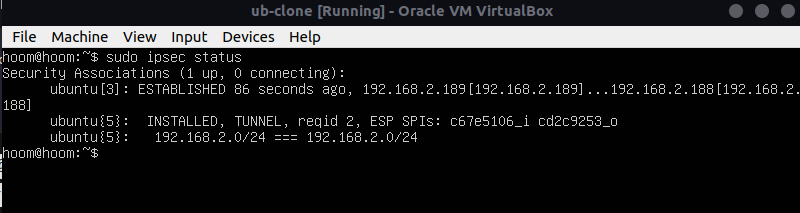
\includegraphics[scale=0.5]{pics/ipsec1.png}
  \end{center}
  \begin{center}
    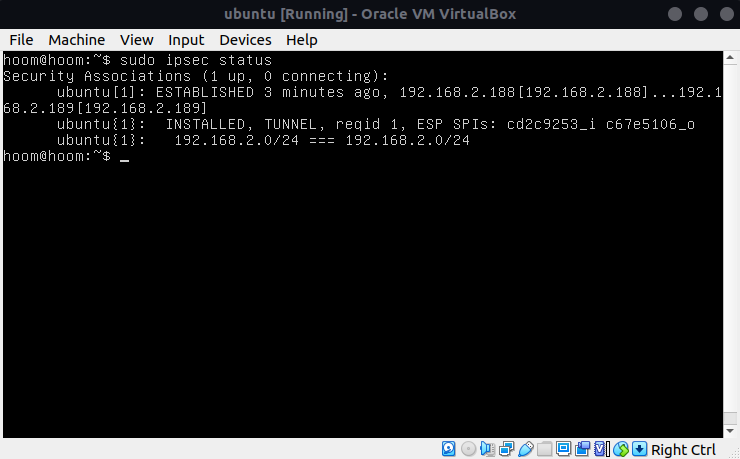
\includegraphics[scale=0.5]{pics/ipsec2.png}
  \end{center}
\end{enumerate}
